\chapter{Preprocessing}\label{preprocessing}

The data downloaded from CrowdTangle and Facebook needs to be preprocessed before we apply it to our proposed methods. The preprocessing steps mainly involve the data collected from the comment section of the food review videos. The comments collected in our research are mainly in three languages- Bangla, English, and Banglish.

To run the BanglaBERT model on the data, we must translate them into Bangla. We follow three basic steps for preprocessing the data. At first, we pass the comment text through 'avro.py', a modern implementation of Avro Phonetic parser \footnote{GitHub: https://github.com/hitblast/avro.py}. The output of the Avro parser is then passed through Google Translate API \footnote{Google Translate API: https://cloud.google.com/translate/}. Even after these two steps, some of the comments were not translated into Bangla. As a result, we had to manually translate the text ourselves. The human-level text filtering steps ensure the quality of data for our research.

\begin{figure}[H]
    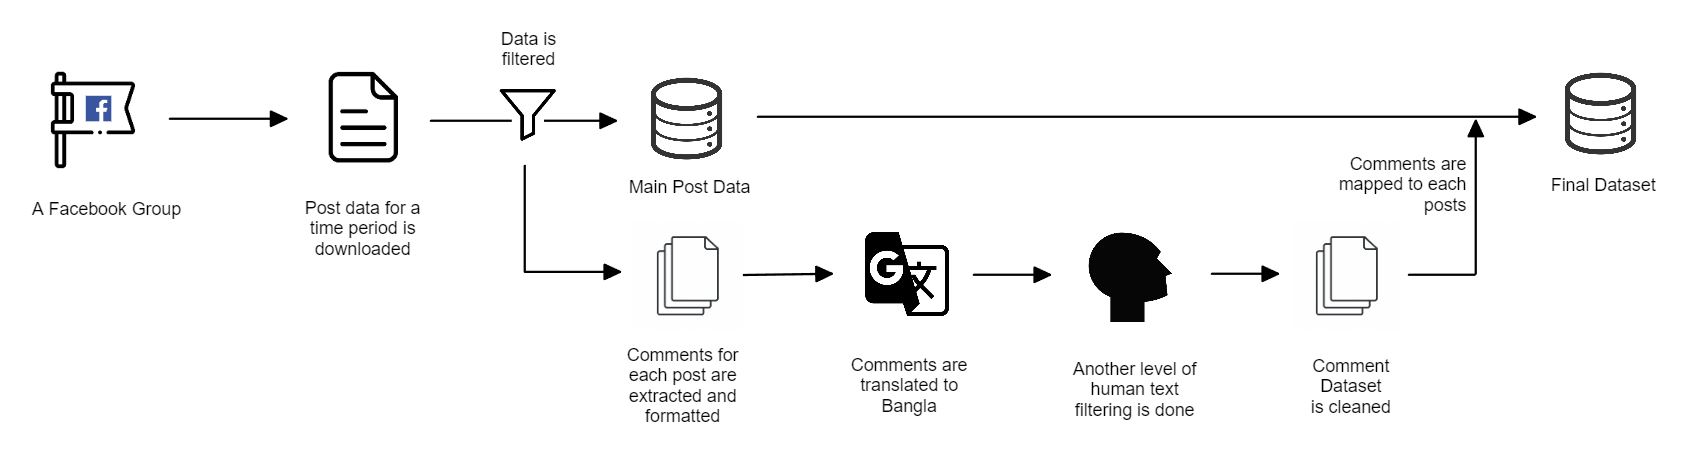
\includegraphics[width=\linewidth]{figures/process.JPG}
    \caption{Data Collection and Pre-processing Steps}
\end{figure}

